%%%%%%%%%%%%%%%%%%%%%%%%%%%%%%%%%%%%%%%%%%%%%%%%%%%%%%%%%%%%%%%%%%%%%%%%%%%%
%% Author template for Transportation Science (trsc)
%% Mirko Janc, Ph.D., INFORMS, mirko.janc@informs.org
%% ver. 0.95, December 2010
%%%%%%%%%%%%%%%%%%%%%%%%%%%%%%%%%%%%%%%%%%%%%%%%%%%%%%%%%%%%%%%%%%%%%%%%%%%%
%\documentclass[trsc,blindrev]{informs3}
\documentclass[trsc,nonblindrev]{informs3} % current default for manuscript submission

\OneAndAHalfSpacedXI % current default line spacing
%%\OneAndAHalfSpacedXII
%%\DoubleSpacedXII
%%\DoubleSpacedXI

% If hyperref is used, dvi-to-ps driver of choice must be declared as
%   an additional option to the \documentclass. For example
%\documentclass[dvips,trsc]{informs3}      % if dvips is used
%\documentclass[dvipsone,trsc]{informs3}   % if dvipsone is used, etc.

% Private macros here (check that there is no clash with the style)

% Natbib setup for author-year style
\usepackage{natbib}
 \bibpunct[, ]{(}{)}{,}{a}{}{,}%
 \def\bibfont{\small}%
 \def\bibsep{\smallskipamount}%
 \def\bibhang{24pt}%
 \def\newblock{\ }%
 \def\BIBand{and}%

%% Setup of theorem styles. Outcomment only one. 
%% Preferred default is the first option.
\TheoremsNumberedThrough     % Preferred (Theorem 1, Lemma 1, Theorem 2)
%\TheoremsNumberedByChapter  % (Theorem 1.1, Lema 1.1, Theorem 1.2)

%% Setup of the equation numbering system. Outcomment only one.
%% Preferred default is the first option.
\EquationsNumberedThrough    % Default: (1), (2), ...
%\EquationsNumberedBySection % (1.1), (1.2), ...

% In the reviewing and copyediting stage enter the manuscript number.
%\MANUSCRIPTNO{} % When the article is logged in and DOI assigned to it,
                 %   this manuscript number is no longer necessary

% postScript packages and setting
\usepackage{graphicx}
\usepackage{ifpdf}
\ifpdf
\DeclareGraphicsExtensions{.pdf,.jpg,.png}
\usepackage[bookmarks=true,colorlinks=true]{hyperref}
\else
\DeclareGraphicsExtensions{.eps}
\usepackage[bookmarks=true,colorlinks=true,dvipdfmx]{hyperref}
\fi
\usepackage{subfigure}

% mathematic packages and settings
% \usepackage{amsmath}
% \usepackage{amssymb}
% \usepackage{amsthm}
\renewcommand{\vec}[1]{#1}
\newcommand{\mat}[1]{#1}
\newtheorem{thm}{Theorem}
\newtheorem{lmm}{Lemma}
\newtheorem{ass}{Assumption}
\newtheorem{rmk}{Remark}
\newtheorem{dfn}{Definition}
\newtheorem{cor}{Corollary}
\newtheorem{prpn}{Proposition}

%%%%%%%%%%%%%%%%
\begin{document}
%%%%%%%%%%%%%%%%

% Outcomment only when entries are known. Otherwise leave as is and 
%   default values will be used.
%\setcounter{page}{1}
%\VOLUME{00}%
%\NO{0}%
%\MONTH{Xxxxx}% (month or a similar seasonal id)
%\YEAR{0000}% e.g., 2005
%\FIRSTPAGE{000}%
%\LASTPAGE{000}%
%\SHORTYEAR{00}% shortened year (two-digit)
%\ISSUE{0000} %
%\LONGFIRSTPAGE{0001} %
%\DOI{10.1287/xxxx.0000.0000}%

% Author's names for the running heads
% Sample depending on the number of authors;
% \RUNAUTHOR{Jones}
% \RUNAUTHOR{Jones and Wilson}
% \RUNAUTHOR{Jones, Miller, and Wilson}
% \RUNAUTHOR{Jones et al.} % for four or more authors
% Enter authors following the given pattern:
%\RUNAUTHOR{}

% Title or shortened title suitable for running heads. Sample:
% \RUNTITLE{Bundling Information Goods of Decreasing Value}
% Enter the (shortened) title:
%\RUNTITLE{}

% Full title. Sample:
% \TITLE{Bundling Information Goods of Decreasing Value}
% Enter the full title:
\TITLE{Thermodynamic Point of View for Urban Transportation Network}

% Block of authors and their affiliations starts here:
% NOTE: Authors with same affiliation, if the order of authors allows, 
%   should be entered in ONE field, separated by a comma. 
%   \EMAIL field can be repeated if more than one author
\ARTICLEAUTHORS{%
\AUTHOR{Huide Zhou, Rachid Bouyekhf, Adbellah EL Moudni}
\AFF{Laboratoire Syst\`{e}mes et Transports (SeT), 
Universit\'{e} de Technologie de Belfort-Montb\'{e}liard (UTBM),
Belfort 90010, France,
\EMAIL{huide.zhou@utbm.fr}, \EMAIL{rachid.bouyekhf@utbm.fr}, \EMAIL{abdellah.el-moudni@utbm.fr}}
% Enter all authors
} % end of the block

\ABSTRACT{%
The paper  explores the application of thermodynamic  formalism to transportation
network. In particular, by considering
the vehicles as the abstract energy supplied to the system, we show in
certain circumstances that  certain thermodynamic
concepts such as  temperature, thermal capacity, thermal
equilibrium can have the corresponding notions in transportation
context. In addition, despite the lack  of the existence  of a natural principle in transportation context that corresponds to the second law of thermodynamics as we will show,  the most important
thermodynamic notion, which is the entropy, can be also defined in
order to measure the disorder of transportation systems.
Then, we show that the thermal equilibrium arising in isolated
thermodynamic system can be also introduced to correspond to
the state when all lanes share the same occupancy. This equilibrium
occupancy leads to a minimum entropy which corresponds to a minimal
disorder.
Finally, by taking the transportation entropy as the storage function,
a dissipativity based control strategy   is presented, by 
means of the Linear Matrix Inequalities (LMI),  to reduce the disorder and
render the system better organized. % Enter your abstract
}%

% Sample
%\KEYWORDS{deterministic inventory theory; infinite linear programming duality; 
%  existence of optimal policies; semi-Markov decision process; cyclic schedule}

% Fill in data. If unknown, outcomment the field
\KEYWORDS{Transportation systems; thermodynamic systems;  entropy;
dissipativity theory; Linear Matrix Inequality (LMI).}
% \HISTORY{}

\maketitle
%%%%%%%%%%%%%%%%%%%%%%%%%%%%%%%%%%%%%%%%%%%%%%%%%%%%%%%%%%%%%%%%%%%%%%

% Samples of sectioning (and labeling) in TRSC
% NOTE: (1) \section and \subsection do NOT end with a period
%       (2) \subsubsection and lower need end punctuation
%       (3) capitalization is as shown (title style).
%
%\section{Introduction.}\label{intro} %%1.
%\subsection{Duality and the Classical EOQ Problem.}\label{class-EOQ} %% 1.1.
%\subsection{Outline.}\label{outline1} %% 1.2.
%\subsubsection{Cyclic Schedules for the General Deterministic SMDP.}
%  \label{cyclic-schedules} %% 1.2.1
%\section{Problem Description.}\label{problemdescription} %% 2.

% Text of your paper here

\section{Introduction}

When we want to study the transportation network, we instantly meet
computational difficulties that grow if the scale of the systems
increases. This situation prevents us from obtaining a clear view of
the influence of various factors on the behavior of the whole system.
The analysis of transportation systems can be obtained in various
ways, depending on the complexity of the problem, but the primary
objective is to reduce computational efforts and to develop
techniques that can be easily implemented on a computer, to allow
automatic analysis of modeled systems. This situation has motivated
many researchers to develop methods and techniques in order to
circumvent difficulties involved in transportation systems. In
particular, the traffic flow theory has been the most widely used
\citep{nathan_h_gartner_revised_2005}. It considers the vehicle
movements as liquid flows, which matches the general impression of
the traffic in modern cities. Hence, the traffic flow theory can
effectively describe the macroscopic traffic phenomenons and has led
to several well-known traffic signal control strategies, like TRANSYT
\citep{hale_traffic_2005}, SCOOT \citep{bretherton_r_d_scoot_1982},
TUC \citep{diakaki_multivariable_2002,papageorgiou_review_2003}, etc.
More precisely, to describe the behavior of such flows, the traffic
flow theory consists of various approaches. Among them, the queueing
theory has been applied to study the behavior of traffic flows near
certain sections (e.g. traffic bottlenecks) where demand exceeds
available capacity \citep{Vandaele2000}. The human factors have been
also concerned in traffic flow theory. Specially, the car following
model examines the manner in which individual vehicles follow one
another \citep{Gipps1981,Zhao2005}. This approach connects the
microscopic behavior of individual vehicles and the macroscopic
features of traffic flows. In addition, the kinematic wave theory has
been very popular to study the flow-density relationship from
microscopic point of view
\citep{zhang_kinematic_2002,jin_multicommodity_2004}. Its first-order
approximation has led to the Cell Transmission Model (CTM)
\citep{daganzo_cell_1995}, which shows high accuracy in the
simulation. Hence, CTM has been used in traffic estimation
\citep{CanudasdeWit2012} and traffic signal control
\citep{Pohlmann2010}. Beside the traffic flow theory, the
applications of Petri nets (PNs) in modeling and control of
transportation systems have been also conducted for over a decade
\citep{ng_review_2013}. This tool is useful for analyzing
performances and assisting intelligent traffic control.

In this paper, we propose another way to study transportation network
which, to the best of our knowledge,  has not been explored yet.
Indeed, by regarding the vehicles as the abstract energy supplied to
the network, we show that certain thermodynamic concepts can be
applied to transportation systems. Among them, the most important
notion is the entropy which measures system disorder and hence can be
taken as a means to evaluate system performances.

This paper is organized as follows: Section \ref{sec:concepts} will
show the connections between transportation and thermodynamic
systems. In particular, the basic concepts such as energy,
temperature, thermal capacity can be introduced into the
transportation context. Then, Section \ref{sec:entropy} will
demonstrates that the transportation system can have a similar notion
of entropy to measure the system disorder.
Section \ref{sec:equilibrium} will show that the thermal equilibrium
can be also introduced to correspond to the state when all lanes share
the same occupancy.
Finally, by considering the transportation entropy as the storage
function, a dissipativity phenomenon will be presented in Section
\ref{sec:dissipativity} to reduce the disorder and hence render the
system better organized.

\section{Basic Concepts and Conservation of Vehicles}\label{sec:concepts}

\subsection{Introduction to Transportation System}

For a transportation system, the connected traffic streets provide a
network such that the vehicles can travel from their departure points
to their destinations. A street is a linear traffic area connecting
two separate points with a fixed length. When more than two streets
meet in a single point, there will be a crossing area among these
streets. These crossing areas and the connected streets compose the
intersections \citep{papageorgiou_review_2003}. For example, Figure
\ref{fig:int4leg} and Figure \ref{fig:int3leg} illustrate two common
types of intersections, which connects 4 and 3 streets respectively.

\begin{figure}[ht]
  \centering
  \subfigure[Four streets]
  {\includegraphics{pics/int4leg}\label{fig:int4leg}}\quad
  \subfigure[Three streets]
  {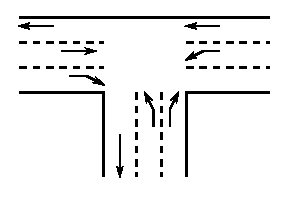
\includegraphics{pics/int3leg}\label{fig:int3leg}}
  \caption{Examples of intersections}
\end{figure}

Based on the directions of vehicles, a street can be further
separated into several traffic lanes. For example, the 4 streets in
the intersection illustrated by Figure \ref{fig:int4leg} are all
split into two lanes corresponding to two opposite directions. On the
other hand, in Figure \ref{fig:int3leg}, all streets  consist of
three lanes (Note that in this intersection, the lanes are split
based on both the current and the potential directions of vehicles).
A street may correspond to more than one traffic signals, but a lane
can only correspond to one. Hence, the traffic lanes are more
appropriate to be considered as the units of the traffic areas
rather than  the streets. For each lane, we choose the number of the
vehicles within it as its state variable. By applying the traffic
flow theory \citep{nathan_h_gartner_revised_2005}, for each lane, the
dynamic of the number of vehicles depends on the traffic flows
connected with this lane.

Now, consider a transportation network including $n$ traffic lanes,
$n>0$. Figure \ref{fig:flows} illustrates all traffic flows related
with the lane $i$, $i\in\{1,\cdots,n\}$. $x_i$ is the number of
vehicles within the lane $i$ at the
beginning of the interval $k$; the flow $r_i$ denotes the vehicles
entering the lane $i$ from the outside; the flow $\sigma_{i,j}$
(resp, $\sigma_{j,i}$), $j\neq i$, $j\in\{1,\cdots,n\}$, represents
the vehicles travel from the lane $j$ (resp, $i$) to the lane $i$
(resp, $j$); the flow $d_{i}$ is the output flow denoting the
vehicles which leave the transportation system from the lane $i$.

\begin{figure}[ht]
  \centering
  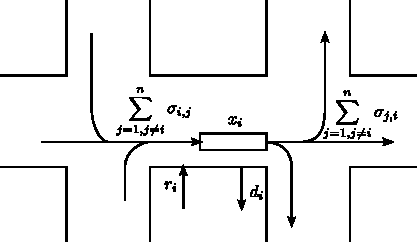
\includegraphics{pics/flows}
  \caption{The traffic flows related with the lane $i$}
  \label{fig:flows}
\end{figure}

Hence, the change of $x_i$ during the interval
$k$, $k\in\mathbb{N}$, is given by
\begin{equation}\label{equ:mdl_gnl_lane}
\Delta x_i(k) = l_i(\vec{x}(k))+r_i(k)-d_i(\vec{x}(k))
\end{equation}
where $\vec{x}=[x_1,\cdots,x_n]^T$ and $l_i$ is the sum of all exchange flows related with lane $i$,
which means
\begin{equation}\label{equ:exchange_vehicle}
 l_i(\vec{x}(k))=\sum_{j=1,j\neq i}^{n}(\sigma_{i,j}(\vec{x}(k))-\sigma_{j,i}(\vec{x}(k)))
\end{equation}
It is important to note that, only the terms corresponding to actual
links between lanes  of the network are made explicit in  equation
\eqref{equ:exchange_vehicle}. Otherwise, all the $\sigma_{i,j}$ for
non-existing links do not appear in the equations.


The model \eqref{equ:mdl_gnl_lane} makes sense only if the state
variables $x_i(k)$ remain non-negative for all $k\in \mathbb{N}$. The
flows $r_i$, $d_{i}$ and $\sigma_{i,j}$ are also defined
to be non-negative on the non-negative orthant. Moreover, it is
obvious that  $\sigma_{i,j}(\vec{x})=0$ and $d_{j}(\vec{x})=0$ if and only if
$x_j=0$, $j\in\{1,\cdots,n\}$. This implies that if the $j$th lane
possesses no vehicles, then it cannot dissipate vehicles to its
surroundings. Conversely, if the $j$th lane does not dissipate
vehicles to its surroundings, then this lane has no vehicle.

Equivalently, in vector form, the transportation system can be
represented by the following state-space difference equation
\begin{equation}\label{equ:mdl_gnl}
\vec{x}(k+1)=\vec{x}(k)+\vec{l}(\vec{x}(k))+\vec{r}(k)-\vec{d}(\vec{x}(k)),\quad \forall k\in\mathbb{N}
\end{equation}
where $\vec{l}=[l_1,\cdots,l_n]^T$,
$\vec{r}=[r_1,\cdots,r_n]^T$, $\vec{d}=[d_1,\cdots,d_n]^T$.

It is important to note that without any specific assumption,
\eqref{equ:mdl_gnl} is a general model, which fits any kind of
transportation system in any circumstance. Based on this general
model, we will explore the nature of transportation system from
thermodynamic point of view in the sequel.

\subsection{Introduction to Thermodynamic System}

The fundamental concept for analyzing   thermodynamic
systems is the concept of energy. Indeed, assume that a matter with
an unique temperature is called a subsystem, the thermodynamic system
consists of a set of connected subsystems. Each of them can store
certain quantity of energy and exchange energy with other subsystems.
Let the energy stored by the subsystems be their state variables. The
dynamic of these states is determined by the energy flows between the
subsystems and their surroundings.

Now, according to the discrete-time thermodynamic model presented by
\citet{haddad_thermodynamic_2005}, consider a thermodynamic system
including $n$ subsystems as shown in Figure \ref{fig:Ther_Sys}. The
$i$th subsystem is denoted by $\Psi_i$, $i\in \{1,\cdots,n\}$, and
its stored energy is denoted by $E_i$. Let $E_i^*>0$ be the thermal
capacity of $\Psi_i$, then the temperature of $\Psi_i$ is given by
\begin{equation}\label{equ:temperature}
    T_i= {E_i}/{E^*_i}
\end{equation}

\begin{figure}[ht]
  % Requires \usepackage{graphicx}
  \centering
  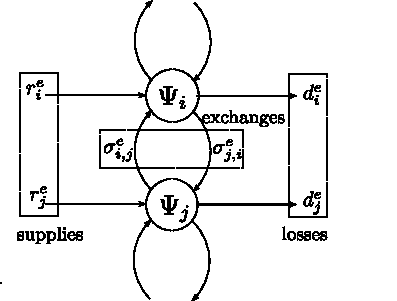
\includegraphics{pics/HModel}
  \caption{Thermodynamic system}
  \label{fig:Ther_Sys}
\end{figure}

In Figure \ref{fig:Ther_Sys}, the energy flow supplied by the outside
to $i$th subsystem is denoted by $r^e_i$. The flow $\sigma^e_{i,j}$
(resp, $\sigma^e_{j,i}$), $i\neq j$, $i,j\in \{1,\cdots,n\}$,
represents the transmission of energy from the $j$th (resp, $i$th)
subsystem to the $i$th (resp, $j$th) subsystem. The flow $d^e_i$,
$i\in \{1,\cdots,n\}$, represents the energy loss from the $i$th
subsystem to the outside of the system. By combining the input,
exchange and output energy flows, the dynamic of the energy $E_i$
stored by $\Psi_i$ can be given by
\begin{equation}\label{equ:Ther_Model_SubSystem}
\Delta E_i(k) = \sum_{j=1,j\neq
i}^{n}(\sigma^e_{i,j}(k)-\sigma^e_{j,i}(k))+r^e_i(k)-d^e_i(k)
\end{equation}
which equivalently infers the state-space model of the thermodynamic
system
\begin{equation}\label{equ:Ther_Model}
    \vec{E}(k+1)=\vec{E}(k)+\vec{l}^e(k)+\vec{r}^e(k)-\vec{d}^e(k)
\end{equation}
where $\vec{E}(k)=[E_1(k),\cdots,E_n(k)]^T$ is the vector of the
energy stored by all subsystems at the beginning of $k$th interval,
$\vec{r}^e=[r^e_1,\cdots,r^e_n]^T$,
$\vec{d}^e=[d^e_{1},\cdots,d^e_{n}]^T$, and
$\vec{l}^e=[l^e_1,\cdots,l^e_n]^T$ represents all exchange flows such
that
\begin{equation*}
l^e_i = \sum_{j=1,j\neq i}^{n}
        (\sigma^e_{i,j}-\sigma^e_{j,i}),
\; i\in \{1,\cdots,n\}
\end{equation*}

\subsection{Correspondences of Basic Concepts}

Now, by comparing the transportation model \eqref{equ:mdl_gnl} and
the thermodynamic model \eqref{equ:Ther_Model}, it is clear that
these two systems have many common aspects. In particular, the
vehicles perform very similarly as the energy does in the
thermodynamic system. Hence, the vehicles can be considered as the
transportation ``energy''. Based on this fundamental correspondence,
the thermodynamic concepts can be introduced into the transportation
context.

Indeed, each traffic lane can contain certain amount of vehicles. The
vehicles move between the connected lanes or between a lane and the
outside. Obviously, the lanes are like the subsystems in the
thermodynamic context, which store energy and exchange energy with
their surroundings. Hence, the traffic lane is the corresponding
notion of the thermodynamic subsystem and the vehicle number $x_i$
corresponds to the energy stored in subsystems $E_i$,
$i\in\{1,\cdots,n\}$.

The temperature is also an important thermodynamic concept. For
finding its correspondence in transportation context, the
corresponding notion of the thermal capacity should be firstly
determined. Since the lengths of traffic lanes are fixed, there
exists a maximal capacity for each lane to contain vehicles. Let
$x_i^*$, $i\in\{1,\cdots,n\}$, be the capacity of the lane $i$. It is
not difficult to observe that the appropriate corresponding notion of
the thermal capacity $E_i^*$ is the lane capacity $x_i^*$.
Furthermore, we can define the occupancy of a lane as the proportion
of the vehicle number to the capacity, which is given by
\begin{equation}\label{equ:occupancy}
f_i = \frac{x_i}{x_i^*},\quad i\in\{1,\cdots,n\}
\end{equation}
Compared with the equation \eqref{equ:temperature}, the occupancies
$f_i$ obviously correspond to the temperatures $T_i$,
$i\in\{1,\cdots,n\}$.

In summary, Table \ref{tab:notions} lists the correspondences of the
basic concepts between thermodynamic and transportation systems. This
analogy will provide us the opportunity to introduce thermodynamic
principles into transportation context as well.

\begin{table}[ht]
\centering \caption{Correspondence of basic concepts}
\label{tab:notions}
\begin{tabular}{cc}
  \hline
  % after \\: \hline or \cline{col1-col2} \cline{col3-col4} ...
  Thermodynamic Concepts & Transportation Concepts \\
  \hline
  energy & vehicles \\
  subsystem & traffic lane \\
  energy stored in a subsystem & number of vehicles in a lane \\
  thermal capacity & lane capacity \\
  temperature & occupancy \\
  \hline
\end{tabular}
\end{table}

\subsection{Conservation of Vehicle (First Principle)}

The first law of thermodynamics, called the conservation of energy
\citep{cengel_thermodynamics:_2001}, indicates that the energy can
not be created or destroyed, it can only change forms or be
transferred. Specially, the change of the energy stored in any
thermodynamic system equals exactly the amount of the net energy
exchange with its surroundings.

This principle also holds for the transportation system, because the
change of vehicles within a system equals exactly the amount of the
net traffic flows between the system and the outside. To show this
principle more clearly, 
let $\vec{\epsilon} \triangleq [1,\cdots,1]^T$ be the vector whose
all components are equal to $1$, and define
\begin{equation}\label{equ:total_vehicle}
U \triangleq \vec{\epsilon}^T\vec{x}=\sum_{i=1}^n x_i
\end{equation}
as the total number of the vehicles within the transportation
network. Let
\begin{equation}\label{equ:all_io}
Q \triangleq \vec{\epsilon}^T(\vec{r}-\vec{d})
\end{equation}
be the number of the net vehicles moving from the outside into the
transportation network. Then, we have $\forall k\in\mathbb{N}$
\begin{equation}\label{equ:conservation}
\Delta U(k) = Q(k)
\end{equation}
where $\Delta U(k)=U(k+1)-U(k)$.
Indeed, from \eqref{equ:mdl_gnl}, we have
\begin{align*}
U(k+1) &= \vec{\epsilon}^T\vec{x}(k+1)\\
       &=
\vec{\epsilon}^T\vec{x}(k)+\vec{\epsilon}^T\vec{l}(\vec{x}(k))
+\vec{\epsilon}^T\Bigl(\vec{r}(k)-\vec{d}(\vec{x}(k))\Bigr)\\
       &= U(k)+\vec{\epsilon}^T\vec{l}(\vec{x}(k))+Q(k)
\end{align*}
It follows
$$\Delta U(k)-Q(k) = \vec{\epsilon}^T\vec{l}(\vec{x}(k))$$
Now, observe that $\vec{\epsilon}^T\vec{l}(\vec{x}(k)) =\displaystyle
\sum_{j=1}^{n} l_i(\vec{x}(k))$ and since 
$$l_i(\vec{x}(k))=\displaystyle\sum_{j=1,j\neq
i}^{n}\Bigl(\sigma_{i,j}(\vec{x}(k))-\sigma_{j,i}(\vec{x}(k))\Bigr)$$
 in view of
\eqref{equ:exchange_vehicle}, it follows
\begin{align*}
\vec{\epsilon}^T\vec{l}(\vec{x}(k))
    &= \sum_{i=1}^n \Bigl(\sum_{j=1,j\neq i}^{n} \sigma_{i,j}(\vec{x}(k))
       -\sum_{j=1,j\neq i}^{n} \sigma_{j,i}(\vec{x}(k))\Bigr)\\
    &= \sum_{i=1}^n \sum_{j=1,j\neq i}^{n} \sigma_{i,j}(\vec{x}(k))
       -\sum_{i=1}^n \sum_{j=1,j\neq i}^{n} \sigma_{j,i}(\vec{x}(k))\\
    &= \sum_{i=1}^n \sum_{j=1,j\neq i}^{n} \sigma_{i,j}(\vec{x}(k))
       -\sum_{j=1}^n \sum_{i=1,i\neq j}^{n} \sigma_{j,i}(\vec{x}(k))\\
    &= 0
\end{align*}
which is the desired result.

This result indicates that the total vehicles in the transportation
system depends only on the traffic flows between the system and the
outside, the exchange flows between different lanes can not change
the total number of the vehicles within the network. Furthermore,
\eqref{equ:conservation} implies
\begin{equation}\label{equ:conservation_ex}
U(k_2) = U(k_1)+\sum_{k=k_1}^{k_2-1}Q(k)
\end{equation}
for any $k_1,k_2\in\mathbb{N}$, $k_2>k_1$. Hence, according to
\citep{willems_dissipative_1972-1}, the conservation of vehicles also
implies that the transportation system \eqref{equ:mdl_gnl} is
lossless with respect to the storage function
\eqref{equ:total_vehicle} and the supply function \eqref{equ:all_io}.

\section{Transportation Entropy}\label{sec:entropy}

\subsection{Second Law of Thermodynamics}

In the thermodynamic system, the directions and the quantities of the
energy movements must follow some specific rules. For example,
without heating equipment, a hot beverage will definitely become
cooler in a cold room. In other words, the energy can not move from
cold air to the hot beverage but in the opposite direction. These
phenomenons are consistent with the second law of thermodynamics
(Clausius statement, \citet{clausius_mechanical_1867}):
\begin{quotation}
\it Heat can never pass from a colder to a warmer body without some
other change, connected therewith, occurring at the same time.
\end{quotation}

This principle is usually connected with a special concept of
\textbf{entropy}. The second law of thermodynamics can be also
described by the way how the entropy of thermodynamic system changes.
In particular, Clausius proposed that the increase of the system
entropy due to the input energy $Q_e$ from the environment is
$Q_e/T^a$, where $T^a$ is the absolute temperature at the spot where
the energy transmission happens \citep{clausius_mechanical_1867}.
However, for any thermodynamic system, the actual increase of entropy
is bigger than or equals to the one supplied by the environment. In
other words, any thermodynamic system is creating entropy itself.
This phenomenon can be presented by the following inequality
\begin{equation}\label{equ:clausius_ther_gnl}
\Delta \psi \ge \int\frac{dQ_e}{T^a}
\end{equation}
or its discrete-time version \citep{haddad_thermodynamic_2005}
\begin{equation}\label{equ:clausius_ther}
\psi(k+1) \ge \psi(k)+\sum_{i=1}^{n}\frac{Q_{ei}(k)}{T^a_i(k+1)},
\forall k\in\mathbb{N}
\end{equation}
where $\psi$ is the entropy of the thermodynamic system, $Q_{ei}(k)$
is the net energy that the $i$th subsystem absorbs from the outside
during the interval $k$, and $T^a_i(k+1)$ is the absolute temperature
of the $i$th subsystem at the end of interval $k$,
$i\in\{1,\cdots,n\}$. \eqref{equ:clausius_ther_gnl} and
\eqref{equ:clausius_ther} are also known as Clausius inequality.

Furthermore, since the entropy is opposite to the capacity of the
thermodynamic system to do useful work, it is also regarded as the
measure of the system disorder \citep{balmakov_entropy_2001}. More
precisely, bigger entropy indicates that the system is worse
organized. Hence, the Clausius inequality also implies that the
thermodynamic system always tends to become worse organized.

For the discrete-time thermodynamic model \eqref{equ:Ther_Model},
based on the Clausius inequality \eqref{equ:clausius_ther},
\citet{haddad_thermodynamic_2005} presented the formula of its
entropy as follows
\begin{equation}
\psi(\vec{E}) \triangleq{\vec{E}^*}^T \ln
(a\vec{\epsilon}+\mat{P}_e\vec{E}) -\vec{\epsilon}^T\vec{E}^*\ln a
\label{equ:Ther_entropy}
\end{equation}
where $\psi(\vec{E})$ is the entropy,
$\vec{E}^*=[E^*_1,\cdots,E^*_n]^T$, $a$ is a positive scalar which
represents the difference between the absolute temperature and the
temperature defined in \eqref{equ:temperature} such that
$T^a_i=a+T_i$, $i\in\{1,\cdots,n\}$, and $\mat{P}_e$ is a diagonal
matrix with diagonal elements $1/E^*_i$. Here, the logarithm of a
vector is the vector of the logarithm of each component.
Note that this formula is identical with the Boltzmann entropy
expression for statistical thermodynamics. 

Since the entropy \eqref{equ:Ther_entropy} is not easy
to apply in control issues, \citet{haddad_thermodynamic_2005} also
introduced a dual notion to entropy, called ectropy, to measure the
system order. The dual inequality to \eqref{equ:clausius_ther} is
given by
\begin{equation}\label{equ:anti_clausius}
\phi(k+1)-\phi(k)\le \sum_{i=0}^n Q_{ei}(k)T_i(k+1),
\forall k\in\mathbb{N}
\end{equation}
where $\phi$ is the ectropy of the thermodynamic system,
$Q_{ei}(k)T_i(k+1)$ is the input ectropy of $i$th subsystem supplied
by the environment with the net input energy $Q_{ei}(k)$, and
$T_i(k+1)$ is the temperature of $i$th subsystem at the end of
interval $k$. This inequality is also called anti-Clausius
inequality, which, like Clausius inequality, is consistent with the
second law of thermodynamics.

Anti-Clausius inequality indicates that in any circumstance, any
thermodynamic system is destroying its ectropy so that the increase
of the ectropy is always less than or equal to the one supplied from
its surroundings. Opposite with the entropy, the ectropy measures the
capacity of the system to do useful work, and bigger ectropy
corresponds to better organization of the system.

For the discrete-time thermodynamic model \eqref{equ:Ther_Model},
based on the anti-Clausius inequality \eqref{equ:anti_clausius},
\citet{haddad_thermodynamic_2005} presented the formula of the
ectropy as follows
\begin{align}
\phi(\vec{E})&\triangleq\frac{1}{2}\vec{E}^T \mat{P}_e \vec{E}
\label{equ:Ther_ectropy}
\end{align}

Contrary to the energy, the entropy and the ectropy are both
non-conservative notions. Specially in the isolated system, the sum
of energy always keeps constant, but the entropy tends to increase
while the ectropy tends to decrease. Besides, it is important to note
that the ectropy \eqref{equ:Ther_ectropy} has the form of Lyapunov
function, which is more useful in control issues than the entropy.

\subsection{Transportation Entropy}
The correspondence between transportation systems and thermodynamic
systems encourages us to introduce the entropy concept into
transportation context in order to evaluate the system performances.
However, the problem is that there is no natural principle in
transportation context that corresponds to the second law of
thermodynamics. As a matter of fact, the directions of vehicles are
determined by the drivers, there is no such rule that the vehicles
only move from more crowded lanes to less crowded ones. Hence, we can
not introduce transportation entropy based on certain principles as
it is defined in the thermodynamic context. Nevertheless, based on
the correspondences of certain concepts, such as energy and
temperature, we can still simply introduce the formulas in the
thermodynamic system to present the transportation entropy as the
measure of the system disorder.

To do this, the significations of orders in these two systems must be
firstly compared. Indeed, in thermodynamic context, higher order
means higher capacity to do useful work, which is related with bigger
temperature differences between subsystems. For example, in a
thermodynamic system including two subsystems, if more energy
concentrates on one single subsystem to generate bigger temperature
difference, the quantity of the potential energy movements is bigger,
which means that the system can generate more useful work. In this
case, the system is regarded as better organized and has higher
order. But on the converse, if the differences between the lane
occupancies are bigger, the order of the transportation system is
lower. Indeed, for a general transportation network, if more vehicles
concentrate in only a few lanes, it has bigger probability to
generate congestions in these lanes and the other lanes are wasted.
In this case, the system is regarded as worse organized and has lower
order.

Moreover, the energy input to the thermodynamic system brings more
capacity to do useful work, which increases the order. However, in
transportation context, the vehicle input brings more potential
opportunity to generate congestions, which decrease the order. For an
isolated thermodynamic system without energy input, the disorder
(entropy) can only increase until it reaches equilibrium. On the
converse, if, at a certain moment, the transportation system has no
vehicle input, the system will keep dissipating the present vehicles
and consequently become better organized.

In conclusion, the order significations of these two systems are
opposite, which means that the disorder in the transportation system
corresponds to the order in the thermodynamic system. In other words,
the transportation entropy (resp, ectropy) should correspond to the
thermodynamic ectropy (resp, entropy). Therefore, according to the
thermodynamic ectropy and entropy formulas \eqref{equ:Ther_ectropy},
\eqref{equ:Ther_entropy}, the \textbf{transportation entropy and
ectropy} are defined respectively as
\begin{align}
\label{equ:Tran_entropy}
\psi(\vec{x}) &\triangleq \frac{1}{2}\vec{x}^T \mat{P} \vec{x}\\
\phi(\vec{x}) &\triangleq{\vec{x}^*}^T \ln
(a\vec{\epsilon}+\mat{P}\vec{x}) -\vec{\epsilon}^T\vec{x}^*\ln a
\label{equ:Tran_ectropy}
\end{align}
where $\psi(\vec{x})$ is transportation entropy, $\phi(\vec{x})$ is
transportation ectropy, $a$ is a positive scalar, $\mat{P}$ is the
diagonal matrix with the diagonal elements $1/x_i^*$, and
$\vec{x}^*=[x_1^*,\cdots,x_n^*]^T$.

The formula of the transportation entropy \eqref{equ:Tran_entropy}
comes only from the thermodynamic system, but we have not shown its
signification in the transportation context. Indeed, the first observation 
  is that if $\vec{x}(k+1)\geq \vec{x}(k)$, then $\psi(\vec{x}(k+1))\geq \psi(\vec{x}(k))$. This implies that 
  when the number of
vehicles of each lane increases between instant $k+1$ and $k$ the entropy  increases as well and hence  the speed of vehicles decreases in each lane that leads to the
greater disorder in the system. Consequently, we can get rise the conclusion that
 the transportation entropy can be thought of as a measure of the system
disorder.

In the case where the numbers of vehicles increase in some lanes while
the ones in the other lanes decrease, we should consider the average
performance of  the entire network to evaluate the
system disorder.
To do this, consider the
transportation network as a service provider and consider the
vehicles traveling within it as its customers. Hence, the order of
transportation network should be the sum of the qualities of the
services provided to all vehicles, and the disorder is, of course,
the opposite. Clearly, the services that vehicles obtain from the
urban transportation system are the traffic routes, and the qualities
are evaluated by how fast the vehicles can pass these routes. Figure
\ref{fig:d_q} shows the flow-density diagram based on kinetic wave
theory, where $\rho_m$ is the jam density, $\nu$ is the speed and
$\nu_m$ is the free-flow speed \citep{ukkusuri_robust_2010}. It is
observed that the traffic flow and the speed can be considered as
functions of the traffic density. More precisely, the bigger traffic
density generates the smaller speed and hence prolongs the delay.
Indeed, despite the habits of drivers, any vehicle need spend more
time to pass more crowded lanes. This indicates that the traffic
density is a parameter for evaluating service quality and hence
bigger density corresponds to the disorder.

\begin{figure}[ht]
  \centering
  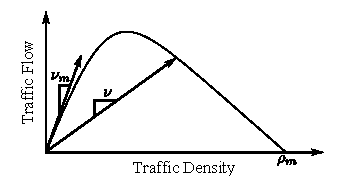
\includegraphics[height=3cm]{pics/d-q}\\
  \caption{Density-flow chart}
  \label{fig:d_q}
\end{figure}

With this in mind, denote the traffic density of the lane $i$ at the
instant $k$ by $\rho_i(k)=x_i(k)/h_i$, where $h_i$ is the length of
the lane $i$. Hence, each vehicle has a density $\rho_i(k)$ as a
service from lane $i$. This is somehow the service that the lane 
provides. Therefore, if $x_i(k)$ is the number of vehicles in lane
$i$, then this lane provides $x_i(k)\rho_i(k)$ services.
Let $I(k)$ be the total service of the network, we have then
\begin{equation}
\label{equ:quality_service}
I(k)=\sum_{i=1}^{n} x_i(k)\rho_i(k)
=\sum_{i=1}^{n}\frac{x_i(k)^2}{h_i}
=\vec{x}(k)^T\mat{P}_h\vec{x}(k)
\end{equation}
where $\mat{P}_h$ is the diagonal matrix with the diagonal elements
$1/h_i$. Note that, since the quality of the service is a decreasing 
function with respect to the density, $I(k)$ is opposite to the
overall quality of the service that the transportation system provides
to all vehicles. In other words, bigger $I(k)$ leads to worse quality of  service.

Now, since $x_i^*=\frac{h_i}{h_{veh}}$ where $h_{veh}$ is the average
car length, it follows
\begin{equation}
I(k) = \sum_{i=1}^{n}\frac{x_i(k)^2}{h_{veh} x_i^*}
= \frac{2}{h_{veh}} \frac{1}{2}\vec{x}(k)^T\mat{P}\vec{x}(k)
= \frac{2}{h_{veh}} \psi(k)
\end{equation}
This indicates that the transportation entropy is proportional to
$I(k)$ and hence it is also opposite to the overall service quality. It
becomes now clear that this transportation entropy is an appropriate
measurement of the system disorder. Indeed, when the total service of
the network  $I(k)$ increases the entropy increases. This
implies that the average speed of vehicles in the network decreases and consequently the
greater disorder in the system.

\section{Occupancy Equilibrium}\label{sec:equilibrium}

For an isolated thermodynamic system without any input
($\vec{r}^e(k)\equiv 0$) and output ($\vec{d}^e(k)\equiv 0$) energy
flows, if a pair of connected subsystems have different temperatures,
the energy transmission will emerge between them so that their
temperatures tend to approximate. After enough amount of time, the
isolated system will reach certain state when the temperature is
spatially and temporally uniform. In this state, the system will lose
all its capacity to produce any useful work. Such particular state is
called thermal equilibrium \citep{cengel_thermodynamics:_2001}. For
an isolated thermodynamic system in thermal equilibrium, its ectropy
would be a minimum and entropy would be a maximum giving rise to a
state of absolute disorder.

Since the lane occupancies correspond to the temperatures, this
concept of thermal equilibrium can be easily introduced into the
transportation context to denote the state when the occupancies of
all traffic lanes are the same. Such state is called the occupancy
equilibrium in this paper. It can be denoted by the following
mathematical expression
\begin{equation}\label{equ:equilibrium}
\frac{\bar{x}_1}{x_1^*}=\cdots=\frac{\bar{x}_n}{x_n^*}=\bar{f}=\text{
constant}
\end{equation}
The occupancy equilibrium implies that no particular concentration of
vehicles exists in the system and hence the possibility to emerge
congestion is extremely low.
% Contrary  to the second law of thermodynamic, for an isolated
% transportation network,
If a transportation network can be isolated in certain circumstances,
its entropy (resp, ectropy) is minimal (resp, maximal) when
the system reaches the occupancy equilibrium. In other words, for
isolated network, this state corresponds to the best organization of
the system. This observation is stated in the following proposition.

\begin{prpn}\label{thm:entropy_equilibrium}
Suppose the transportation network is isolated. Let $N$ be the total
number of vehicles in the system. Let $\psi(\vec{x})$ and
$\phi(\vec{x})$ denote the entropy and ectropy of the system  given
by \eqref{equ:Tran_entropy} and \eqref{equ:Tran_ectropy}
respectively, and define $\mathbb{D}\triangleq
\{\vec{x}\in\mathbb{R}^n_+/\vec{\epsilon}^T\vec{x}=N\}$. Then,
\begin{equation}\label{equ:entropy_equilibrium}
\arg\min_{\vec{x}\in\mathbb{D}}(\psi(\vec{x})) =
\arg\max_{\vec{x}\in\mathbb{D}}(\phi(\vec{x})) = \bar{\vec{x}} =
\frac{N}{\vec{\epsilon}^T\vec{x}^*}\vec{x}^*
\end{equation}
\end{prpn}
\proof{proof:}
The proof is identical to the proof of Proposition 3.17
of \citet{haddad_thermodynamic_2005}. Hence it is omitted here.
\endproof
Now, observe that if the state $ \bar{\vec{x}}$ is reached, then
$\frac{\bar{x}_i}{x_i^*}=\frac{N}{\vec{\epsilon}^T\vec{x}^*}=\bar{f}$,
for all $i=1,\cdots, n$, which corresponds to the occupancy
equilibrium. This occupancy equilibrium leads to the minimal disorder
and maximal order for the transportation network. Hence, the study of
control problems should concern this state as an important objective.

\iffalse
Now, if we assume that $\sigma_{i,j}=\sigma_{j,i}$ if and only if
$\frac{x_i}{x_i^*}=\frac{x_j}{x_j^*}$, then $ \bar{\vec{x}}$  is an
equilibrium state Lyapunov stable. Indeed, since the system is
isolated $S(k)=0$. It follows from equation \eqref{eq:g} that $g(k)=0$
and hence $\Delta\psi(\vec{x}(k))\leq0$ in view of
\eqref{equ:dissipative1}.
\fi

\section{Dissipativity based control of the entropy}
\label{sec:dissipativity}

Now, in transportation context, the input vehicles bring disorder to
the system. This supplied disorder depends not only on  the  net vehicles exchange between the network and the outside  $\vec{r}(k)-\vec{d}(k)$, but also on the distribution of them. The vehicles
which enter the more crowded lanes bring more disorder than the ones
with the same quantity which enter the less crowded lanes. Since the
occupancies represent how the lanes are crowed, it is natural to
measure the supplied entropy with respect to the input flows $\vec{r}(k)-\vec{d}(k)$ and 
occupancy factors. Let $\vec{f}=[f_1,\cdots,f_n]^T$ be the vector of
all occupancies. Note that because $\vec{f}(k)$ corresponds to the
beginning of the interval $k$ while $\vec{f}(k+1)$ corresponds to the
end of it, the supplied entropy in the interval $k$ should be with respect 
to $\vec{f}(k+1)$ rather than $\vec{f}(k)$. So, we define
$$S(k)=\vec{f}^T(k+1)\bigl(\vec{r}(k)-d(k)\bigr)$$
as the supplied entropy in the interval $k$. Furthermore, since
$\vec{f}=\mat{P}\vec{x}$ in view of \eqref{equ:occupancy}, the
supplied entropy is restated as
\begin{equation}\label{equ:supply}
    S(k)=\vec{x}^T(k+1) \mat{P} \bigl(\vec{r}(k)-\vec{d}(k)\bigr)
\end{equation}
Now, as in the anti-Clausius inequality \eqref{equ:anti_clausius}, we
propose its corresponding version in transportation context as
follows
\begin{equation}\label{equ:dissipative}
\psi(\vec{x}(k+1))-\psi(\vec{x}(k)) \leq S(k),\quad \forall
k\in\mathbb{N}
\end{equation}
If this inequality is verified, the transportation system has the
tendency to decrease its disorder and become better organized.

Furthermore, according to the \citet{willems_dissipative_1972} and
\citet{hill_dissipative_1980}, \eqref{equ:dissipative} also implies
the dissipativity of the system with the entropy \eqref{equ:Tran_entropy} as the
storage function and with \eqref{equ:supply} as the supply function.
In this case, \eqref{equ:dissipative} is called the dissipation  
inequality. Figure \ref{fig:trans_dis} illustrates this dissipativity
of system disorder. Indeed, the input flows bring disorder to the
transportation system to make it worse organized. At the same time,
the appropriate traffic signal control dissipates the traffic so that
the system stores only a part of this input disorder.
\begin{figure}[ht]
  \centering
  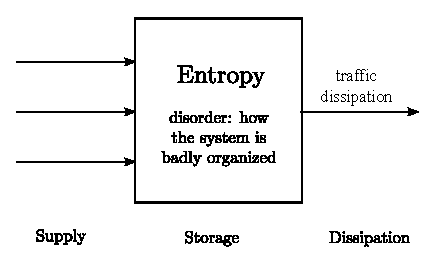
\includegraphics{pics/trans_dis}\\
  \caption{Dissipativity of transportation entropy}
  \label{fig:trans_dis}
\end{figure}

This dissipativity implies that the storage of the system disorder is
always smaller than or equal to the supplied one from the outside. In
other words, if this dissipativity phenomenon exists in the
transportation system, the system disorder will tend to decrease and
hence the system will tend to become better organized. 
However, contrary to thermodynamic systems, this dissipativity does not exist naturally. To show this, 
observe that 
\begin{align*}
\Delta\psi(\vec{x}(k))
&=\frac{1}{2}\vec{x}^T(k+1)\mat{P}\vec{x}(k+1)
-\frac{1}{2}\vec{x}^T(k)\mat{P}\vec{x}(k)\\
&=\vec{x}^T(k+1)\mat{P}
\Bigl(\vec{x}(k+1)-\vec{x}(k)-\vec{l}(k)\Bigr)\\
&-\frac{1}{2}\Bigl(\vec{x}(k+1)-\vec{x}(k)\Bigr)^T
\mat{P}\Bigl(\vec{x}(k+1)-\vec{x}(k)\Bigr)\\
&+\vec{x}^T(k+1)\mat{P}\vec{l}(k)\\
\end{align*}
Since $\mat{P}$ is positive definite and
$\vec{x}(k+1)-\vec{x}(k)-\vec{l}(k)=\vec{r}(k)-\vec{d}(k)$, it follows
\begin{equation}\label{equ:dissipative1}
\Delta\psi(\vec{x}(k))\leq S(k)+\vec{x}^T(k+1)\mat{P}\vec{l}(k)
\end{equation}
Let $g(\vec{x}(k))=\vec{x}^T(k+1)P\vec{l}(k)$ and since
$l_i(k)=\sum_{j=1,j\neq i}^{n}(\sigma_{i,j}(k)-\sigma_{j,i}(k))$, it
follows
\begin{align}\label{eq:g}
g(\vec{x}(k))&=\sum_{i=1}^{n}
\frac{x_i(k+1)l_i(k)}{x_i^*}=
\sum_{i=1}^{n}\sum_{j=1,j\neq i}^{n}
\frac{x_i(k+1)(\sigma_{i,j}(k)-\sigma_{j,i}(k))}{x_i^*}
\nonumber\\
&=\sum_{i=1}^{n-1}\sum_{j=i+1}^{n}
\Bigl(\frac{x_i(k+1)}{x_i^*}-\frac{x_j(k+1)}{x_j^*}\Bigr)
\Bigl(\sigma_{i,j}(k)-\sigma_{j,i}(k)\Bigl)\nonumber\\
 \end{align}
Now, if we suppose that
$\bigl(\frac{x_i(k+1)}{x_i^*}-\frac{x_j(k+1)}{x_j^*}\bigr)
\bigl(\sigma_{i,j}(k)-\sigma_{j,i}(k)\bigl)\le 0$ for all $i\neq j$
and for all $k\in\mathbb{N}$,
then $\Delta\psi(\vec{x}(k)) \leq S(k)$, $\forall k\in\mathbb{N}$, and
hence the transportation system is dissipative. Unfortunately, this 
assumption does not exist in reality because it implies that the more
occupied lanes give  more vehicles to the less occupied ones which is
not realistic in transportation systems. Even the situation where
$\sigma_{i,j}(k)=\sigma_{j,i}(k)$ (lanes $i$ and $j$ have the same  
exchange between them) for all $k\in\mathbb{N}$ is not realistic
either because the directions of vehicles are determined by the
drivers. However, it is known that the traffic signals have the
ability to control the traffic flows.
Therefore, it is possible that under certain control schemes, the
traffic signals can verify the dissipation inequality
\eqref{equ:dissipative} without verifying this assumption. This is the
main concern in the following.

First observe that, if $d_{i}(x)$ is differentiable and since
$d_{i}(x)=0$ if and only if $x_i=0, i=1,\cdots,n$, it can be written
as $d_{i}(x)=\hat{d}_{i}(x)x_i$ with $\hat{d}_{i}(x)\geq0$
\citep{Jacquez1993}.
On the other hand, the exchange traffic flows are determined by the
traffic signals. Indeed, for certain cycle $k$, $\sigma_{i,j}$ can be
considered proportional to the corresponding effective green time
$u_j$ as follows $\forall i,j\in\{1,\cdots,n\}$, $i\neq j$
\citep{papageorgiou_review_2003}
$$\sigma_{i,j}(k)=\lambda_{i,j}(x) s_j(x) u_j(k)$$
where $s_j>0$ is the average rate of leaving flow from lane $j$, and
$\lambda_{i,j}\in[0,1]$ is the turning rate from lane $j$ towards
lane $i$. This infers that
\begin{equation}
\label{eql}
\begin{split}
l_i(k)&=\sum_{j=1,j\neq i}^{n} \sigma_{i,j}(k)
         -\sum_{j=1,j\neq i}^{n} \sigma_{j,i}(k)\\
      &=\sum_{j=1,j\neq i}^{n} s_j(x) u_{j}(k) \lambda_{i,j}(x)
        -\sum_{j=1,j\neq i}^{n} s_i(x) u_{i}(k) \lambda_{j,i}(x)\\
      &=\sum_{j=1,j\neq i}^{n} s_j(x) u_{j}(k) \lambda_{i,j}(x)
        -s_i(x)u_{i}(k)\sum_{j=1,j\neq i}^{n}  \lambda_{j,i}(x)
\end{split}
\end{equation}
Let $\vec{u} = [u_1,\cdots,u_n]^T$ and define a vector
$\vec{B}_i(x)=[B_{i,1}(x),\cdots,B_{i,n}(x)]^T\in\mathbb{R}^{n\times
n}$ in the following manner
\begin{equation*}
 B_{i,j}(x)= \left\{ \begin{array}{l@{\,:\,}r}
            - s_i(x) \sum_{j=1,j\neq i}^{n}  \lambda_{j,i}(x)
            &\quad \text{for}\; i= j\\
              s_j(x) \lambda_{i,j}(x)&\quad
             \text{for}\;i\neq j
            \end{array}\right.
\end{equation*}
Then equation \eqref{eql} can be rewritten as
\begin{equation}
\label{equ:Con_li}
\begin{split}
l_i(k)&=\sum_{j=1,j\neq i}^{n} B_{i,j} u_{j}(k)
        +B_{i,i} u_{i}(k)\\
        &=\sum_{j=1}^{n} B_{i,j} u_{j}(k)\\
      &=\vec{B}_i^T\vec{u}(k)
\end{split}
\end{equation}

Let $\mat{D}(x)=diag\{\hat{d}_{1}(x),\cdots,\hat{d}_{n}(x)\}$,
$\mat{A}(x)=\mat{I}-\mat{D}(x)$ and $\mat{B}(x) =
[\vec{B}_1(x),\cdots,\vec{B}_n(x)]^T$. In this case, the equation
\eqref{equ:mdl_gnl} becomes
$$
\vec{x}(k+1)=\mat{A}(x)\vec{x}(k)+\mat{B}(x)\vec{u}(k)+\vec{r}(k)
$$

Now, the dissipativity based control problem is stated as follows:
find $\vec{u}(x)$ such that the closed loop system is dissipative. In
other words, find $\vec{u}(x)$ such that
\begin{align}\label{pbc0}
g(\vec{u}(k))&=\vec{x}^T(k+1)\mat{P}\vec{l}(k)\nonumber\\
&=\vec{u}^T(k)\mat{B}^T\mat{P}\mat{B}\vec{u}(k)
+\vec{u}^T(k)\mat{B}^T\mat{P}(\mat{A}\vec{x}(k)+\vec{r}(k))\leq 0
\end{align}
In the following, we will provide the way to construct a feedback
control law that achieves the dissipativity. To make the idea clear,
put $\vec{y}=\frac{1}{2}(\mat{A}\vec{x}+\vec{r})$. It follows 
\begin{equation}\label{pbc}
g(\vec{u})=\vec{u}^T\mat{B}^T\mat{P}\mat{B}\vec{u}+2\vec{u}^T\mat{B}^T\mat{P}\vec{y}
\end{equation}
which implies
$$g(\vec{u})=(\mat{B}\vec{u}
+\vec{y})^T \mat{P} (\mat{B}\vec{u}
+\vec{y})-\vec{y}^T
\mat{P}\vec{y}$$
Let $\mat{H}\in\mathbb{R}^{n\times n}$ and put
$\vec{u}=\mat{H}\vec{y}$, we get
$$g(\vec{y})= \vec{y}^T\Bigl[(\mat{B}\mat{H}+\mat{I})^T \mat{P}
(\mat{B}\mat{H}+\mat{I})-\mat{P}\Bigr]\vec{y}
$$
Hence, $\mat{H}$ must be chosen such that the matrix
$(\mat{B}\mat{H}+\mat{I})^T \mat{P}
(\mat{B}\mat{H}+\mat{I})-\mat{P}$ is negative
semidefinite, which is equivalent to
$$\mat{P}-(\mat{B}\mat{H}+\mat{I})^T \mat{P}
(\mat{B}\mat{H}+\mat{I})\succeq 0$$
where $\succeq$ means the matrix is positive semidefinite.
This inequality is equivalent to the following Linear Matrix
Inequality (LMI) by applying the Schur
complement lemma (See Appendix)
$$\begin{pmatrix}
\mat{P}& (\mat{B}\mat{H}+\mat{I})^T \mat{P} \\
\mat{P} (\mat{B}\mat{H}+\mat{I})  & \mat{P}
\end{pmatrix}\succeq 0$$
Summarizing, we have the following theorem. 

\begin{thm}\label{thm:pbc}
For the transportation system, the feedback control law
\begin{equation}
\label{equ:feedback}
\vec{u}=\frac{1}{2}\mat{H}(\mat{A}\vec{x}+\vec{r})
\end{equation}
renders the system dissipative with respect to
entropy \eqref{equ:Tran_entropy} as the storage function and the
supply function \eqref{equ:supply} if $\mat{H}$ is a solution of the
following LMI
\begin{equation}\label{equ:lmi}
\begin{pmatrix}
\mat{P}& (\mat{B}\mat{H}+\mat{I})^T \mat{P} \\
\mat{P} (\mat{B}\mat{H}+\mat{I})  & \mat{P}
\end{pmatrix}\succeq 0
\end{equation}
\end{thm}
This theorem provide a simple way to solve the dissipativity based control problem.
However, since $\mat{B}$ is a function of $\vec{x}$, the LMI \eqref{equ:lmi} should be solved for each cycle to get feedback gain $\mat{H}$. This presents  computational difficulties, which rapidly grow if the scale of the systems increases. To overcome this difficulty, we propose in the sequel a solution for the dissipativity based control problem independent of $B$. To do this, 
let
$\mat{M}=\mat{B}^T\mat{P}\mat{B}$ and
$\vec{y}=\frac{1}{2}\mat{B}^T\mat{P}(\mat{A}\vec{x}+\vec{r})$.  It
follows from Eq. \eqref{pbc0} that
\begin{equation}\label{pbcc}
g(\vec{u})=\vec{u}^T\mat{M}\vec{u}+2\vec{u}^T\vec{y}
\end{equation}
Now, observe that  since $\epsilon^T\vec{l} =\epsilon^T\mat{B}\vec{u}=0$ for all $u$ then $\epsilon^T\mat{B}=0$ which implies that the rows of $B$ are linearly dependent. Consequently  $B$ is singular so  $M$ is symmetric positive semidefinite and  all its eigenvalues  are nonnegative.  Hence, there exists an orthogonal matrix $K$ such that $M=KCK^T $, where $C$ is a diagonal matrix of the form
$$C=diag(\xi_1;\cdots,\xi_r,0,\cdots,0)$$
where $\xi_i>0$  are the positive eigenvalues  of $M$  and $r$ is the rank of $M$ . The orthonormal columns of $K$  are the eigenvectors of all eigenvalues  of $M$. 

Now, let $D =diag(\xi_1;\cdots,\xi_r)$, $D$ is invertible  and $M$ can be rewritten as
$$M=K\left(\begin{array}{cc}D^{\frac{1}{2}}& 0 \\ 0 &I_{n-r} 
\end{array}\right)
\left(\begin{array}{cc}I_r& 0 \\ 0 &0 
\end{array}\right)
\left(\begin{array}{cc}D^{\frac{1}{2}}& 0 \\ 0 &I_{n-r} 
\end{array}\right)
K^T$$
If we put 
$$Q=K\left(\begin{array}{cc}D^{\frac{1}{2}}& 0 \\ 0 &I_{n-r} 
\end{array}\right)$$
then $Q^{-1}$ is well defined because $K$ is orthogonal. Hence, let $z=Q^T u$  and $\theta= Q^{-1}y$, equation \eqref{pbcc} can be rewritten as
\begin{align}\label{pbc1}
g(z)&=z^T\left(\begin{array}{cc}I_r& 0 \\ 0 &0 
\end{array}\right)z+2z^T\theta=z^T z +2z^T \theta -z^T\left(\begin{array}{cc}0& 0 \\ 0 &I_{n-r} 
\end{array}\right) z\nonumber\\
&\leq z^T z +2z^T \theta=(z+\theta)^T (z+\theta) -\theta^T \theta
\end{align}
Let $R\in\mathbb{R}^{n\times n}$ and put
$z=R\theta$, it follows
\begin{equation}\label{pbc2}
f(\theta)=(z+\theta)^T (z+\theta) -\theta^T \theta=\theta^T\Bigl[(R+I)^T(R+I)-I\Bigr]\theta
\end{equation}
Hence, $f(\theta)\leq 0$ for all $\theta$  if and only if
$(R+I)^T(R+I)-I$  is negative semidefinite, which is equivalent to 
  the following LMI 
$$\begin{pmatrix}
\mat{I}& (\mat{R}+\mat{I})^T  \\
 (\mat{R}+\mat{I})  & \mat{I}
\end{pmatrix}\succeq 0$$
This LMI is now independent of $\vec{x}$, hence it can be solved once for all cycles. Summarizing, we have the following theorem. 

\begin{thm}\label{thm:pbc2} Let $R$  be a solution of the
following LMI
$$\begin{pmatrix}
\mat{I}& (\mat{R}+\mat{I})^T  \\
 (\mat{R}+\mat{I})  & \mat{I}
\end{pmatrix}\succeq 0$$
Then, for the transportation system, the feedback control law
\begin{equation}
\label{equ:feedback2}
\vec{u}=\frac{1}{2}(\mat{Q}^T)^{-1}\mat{R}\mat{Q}^{-1}\mat{B}^T\mat{P}(\mat{A}
\vec{x}+\vec{r})
\end{equation}
renders the system dissipative with respect to
entropy \eqref{equ:Tran_entropy} as the storage function and the
supply function \eqref{equ:supply}.\end{thm}


Now, observe that if the matrix $R$ is chosen to be symmetric then $f(\theta)\leq 0$ if and only if $-2\leq\lambda_i\leq 0$, for each  eigenvalue $\lambda_i$  
 of $R$. To show this, it suffices to observe that because $R$ is symmetric it is always diagonalizable. Let $R=FLF^T$ be the eigendecomposition of $R$, where $F^T=F^{-1}$ and $L$ is the diagonal matrix whose diagonal elements are the  eigenvalues of $R$. We have 
 $$(R+I)^T(R+I)-I=R^2+2R=F(L^2+2L)F^T$$
It follows that $f(\theta)\leq 0$ if and only if $(L^2+2L)$ is negative semidefinite. Since $L^2+2L=diag(\lambda_1^2+2\lambda_1,\cdots,\lambda_n^2+2\lambda_n)$, it follows $(L^2+2L)$ is negative semidefinite if and only if  $\lambda_i^2+2\lambda_i \leq 0, \forall i $. This infers that  $-2\leq\lambda_i\leq 0$.

In the particular situation where $\mat{R}=r\mat{I}$, $r\in
\mathbb{R}$,
for any vector $\vec{\theta}$, $f(\vec{\theta})$ is non-positive if and only if $-2\leq r\leq 0$. Summarizing, we have the following corollary. 

\begin{cor}\label{thm:pbcc2} Let $R$ be a symmetric matrix such that $-2\leq\lambda_i\leq 0,  \forall
i=1,\cdots,n$, where $\lambda_i$ is an eigenvalue of $R$. Then 
 the feedback control law
\begin{equation}
\label{equ:feedback2bis}
\vec{u}=\frac{1}{2}(\mat{Q}^T)^{-1}\mat{R}\mat{Q}^{-1}\mat{B}^T\mat{P}(\mat{A}
\vec{x}+\vec{r})
\end{equation}
renders the system dissipative with respect to
entropy \eqref{equ:Tran_entropy} as the storage function and the
supply function \eqref{equ:supply}.
 
\end{cor}

From the corollary just stated,  it follows immediately that, for any
arbitrarily selected $R$ that satisfies $-2\leq\lambda_i\leq 0,  \forall i=1,\cdots,n$, the feedback
control defined by \eqref{equ:feedback2bis} exhausts the class of control laws
which render the system dissipative. Hence, corollary \ref{thm:pbcc2} 
gives explicit but non-unique solutions of the the dissipativity based
control problem.

Furthermore, the application of the control $\vec{u}$ in real
transportation systems must concern the physical limitations on the
traffic signals. For example, if the constraint on $\vec{u}$ is given
by
$$u_{i,min}\le u_i\le u_{i,max},\quad i\in\{1,\cdots,n\}
$$
then one possible solution is to apply the following saturation
function
\begin{equation}
sat(u_i) = \left\{ \begin{array}{l@{\quad:\quad}c}
        u_{i,min} & u_i\le u_{i,min}\\
        u_i & u_{i,min}\le u_i\le u_{i,max}\\
        u_{i,max} & u_i\ge u_{i,max}
        \end{array}\right.
\end{equation}
where $u_i$ is the value derived from the feedback
\eqref{equ:feedback}, and $sat(u_i)$ is the actual control applied
to real system.



\section{Conclusion}

This paper has tried  to present a thermodynamic point of view for the
transportation network. Indeed, the comparison between thermodynamic
and transportation systems has shown that they are very similar by
regarding the vehicles as the abstract energy supplied to the
system and regarding the traffic lanes
as the thermodynamic subsystems. In addition, the concepts of thermal
capacity and temperature are also introduced into transportation
context to correspond to lane capacity and occupancy respectively.
Then, it has been demonstrated that the first law of thermodynamics
corresponds to the conservation of vehicles.

However, though these two kinds of systems can be similar, the second
thermodynamic principle does not work in transportation context. The
reason for this is that  the directions of vehicles are determined by
the drivers, there is no rule that the vehicles only move from more
crowded lanes to less crowded ones. Besides, the significations of
order in two systems are opposite, which means that the thermodynamic
ectropy corresponds to the transportation entropy. Such
transportation entropy is a measure of disorder of the system and
hence may provide deep insight in the analysis of transportation
control problems.
In particular, this paper has presented a dissipassivity phenomenon
of transportation entropy that reduces the system disorder and hence
renders the system better organized.
Though this phenomenon doesn't exist naturally in transportation
context, the ways to construct feedback control strategies have been
proposed  to achieve such objective by means of Linear Matrix Inequalities (LMI).

Finally, we would like to point out that, the traffic lanes
are chosen as the units of transportation systems in this paper, the
thermodynamic point of view can also be applied to other units of
analysis, e.g intersections or road segments. This may enable us to
study other transportation phenomenons like lane-changing, routing,
etc in the future.

% Appendix here
% Options are (1) APPENDIX (with or without general title) or 
%             (2) APPENDICES (if it has more than one unrelated sections)
% Outcomment the appropriate case if necessary
%
\begin{APPENDIX}{}

According to \citep{boyd_linear_1994}, a linear matrix inequality (LMI) is an expression of the form
$$F(x)\triangleq F_0+\sum_{i=1}^m x_iF_i \succ 0$$
where $x\in\mathbb{R}^m$ and the symmetric matrices $F_i=F_i^T\in\mathbb{R}^{n\times n}$, $i=0,\cdots,m$, are given. The symbol $\succ$ means that $F(x)$  is positive definite.
The non-strict LMI can be also defined as
$$F(x)\succeq 0$$

The LMI represents a wide variety of convex constraints on $x$ because linear inequalities, quadratic inequalities, matrix norm inequalities, etc can all be cast into the form of LMI.
In particular, nonlinear but convex inequalities are converted to LMI usually by using the following Schur complement lemma.

\begin{lmm}
Let $S$ be a symmetric matrix of the form
$$S=\begin{pmatrix}
     A&B^T\\B&C
    \end{pmatrix}
$$
and $C$ is invertible. Then $S\succeq 0$ if and only if $C\succ 0$
and $A-B^TC^{-1}B\succeq 0$.
\end{lmm}

\end{APPENDIX}
%
%   or 
%
% \begin{APPENDICES}
% \section{<Title of Section A>}
% \section{<Title of Section B>}
% etc
% \end{APPENDICES}


% References here (outcomment the appropriate case) 

% CASE 1: BiBTeX used to constantly update the references 
%   (while the paper is being written).
\bibliographystyle{ormsv080} % outcomment this and next line in Case 1
\bibliography{zhou_refs} % if more than one, comma separated

% CASE 2: BiBTeX used to generate mypaper.bbl (to be further fine tuned)
%\input{mypaper.bbl} % outcomment this line in Case 2

\end{document}
